\chapter{Simulazione}
Per valutare le prestazioni del sistema realizzato si sono effettuate numerose simulazioni. Tutti i test condotti sono stati basati su una specifica configurazione di nodi, in particolare 1 nodo Publisher e 2 Subscriber. I due nodi consumer richiedono la stipulazione di un contratto al producer, il quale espleta tutte le richieste. Si riporta ora un esempio di esecuzione con relativa descrizione ed analisi dei dati.
\section{Esecuzione}
In principio si avvia il nodo Producer il quale andrà in attesa di richieste dei consumatori. In seguito si avviano i due Consumer (o Subscriber) i quali richiedono ed ottengono un contratto con il Subscriber. Stabiliti i contratti inizia la vera fase di simulazione in cui ogni nodo genera valori casuali per le proprie risorse e lo SC raccoglie tali dati per valutare gli SLA e la necessità di migrazione.
\subsection{Scenario}
I tre nodi dello scenario d'esecuzione hanno le seguenti caratteristiche:
\begin{enumerate}
	\item Publisher con connessione WIRED e 512Kb di banda;
	\item subscriber con connessione WIRELESS e 256Kb di banda;
	\item subscriber con connessione WIRELESS e 256Kb di banda.
\end{enumerate}
\subsection{Generazione contratti SLA}
Il contratto SLA, ovvero i livelli di latency, reliability e reqInterval vengono generati casualmente dal publisher nel momento in cui raccolgono una richiesta di contratto. Tale operazione può essere vista nel log di esecuzione del programma simulativo.
\begin{enumerate}
\item Il Subscriber richiede un contratto con un qualsiasi publisher disponibile;
\item Il publisher legge la richiesta dal dsm;
\begin{center}
\begin{verbatim}
SLAContract-request received from cm2
\end{verbatim}
\end{center}
\item il publisher genera i parametri del contratto casualmente e lo immette sul dsm;
\item lo SC rileva la presenza del contratto e lo aggiunge alla sua lista.
\begin{center}
\begin{verbatim}
Added Contract
\end{verbatim}
\end{center}
\end{enumerate}
\subsection{Migrazione}
Inizialmente lo SC risiede sul primo nodo, ovvero il publisher (ved. \ref{fig:primo}).
\begin{figure}[H]
\begin{center}
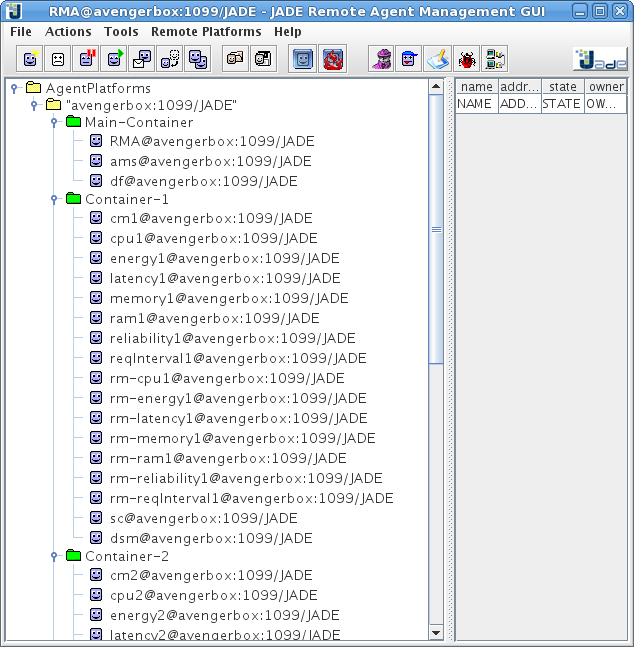
\includegraphics[scale=0.5]{etc/primo.png}
\caption{Migrazione non avvenuta}
\label{fig:primo}
\end{center}
\end{figure}
In questa figura si può notare la presenza del dsm e dello SC sul primo nodo, in quanto la simulazione è stata appena avviata. Dal log si può rilevare che lo SC ha già iniziato a controllare la necessità di migrazione e che al momento si trova sul Container-1 ovvero il nodo 1. Il valore index del nodo attuale non ha ancora superato il valore di soglia (52), di conseguenza lo SC rimane sul nodo attuale.
\begin{lstlisting}
Sono su Container-1
Context[cm3]--> cpu: 21.126825, ram: 12.573414, memory: 35.398045, energy: 64.588715, index: 26.515991
Context[cm1]--> cpu: 78.77115, ram: 63.975082, memory: 15.567526, energy: 100.0, index: 36.412167
Context[cm2]--> cpu: 50.302402, ram: 11.7872715, memory: 1.3100842, energy: 91.46843, index: 17.141415
Associated with: cm1
Actual context--> cpu: 78.77115, ram: 63.975082, memory: 15.567526, energy: 100.0, index: 36.412167
\end{lstlisting}
Nel momento in cui il carico su tale nodo raggiunge valori troppo alti avverrà la migrazione. Infatti poco tempo dopo si ha una situazione del genere:
\begin{lstlisting}
Sono su Container-1
Context[cm3]--> cpu: 10.354793, ram: 26.346369, memory: 2.7747908, energy: 75.6174, index: 16.394249
Context[cm1]--> cpu: 77.09479, ram: 64.88432, memory: 87.20903, energy: 100.0, index: 52.713272
Context[cm2]--> cpu: 5.725228, ram: 59.014675, memory: 7.089407, energy: 92.148476, index: 18.876198
Associated with: cm1
Actual context--> cpu: 77.09479, ram: 64.88432, memory: 87.20903, energy: 100.0, index: <52.713272>
Migration to cm3
Moving DSM to 3

Sono su Container-3
Context[cm1]--> cpu: 7.0192904, ram: 18.302485, memory: 86.83973, energy: 100.0, index: 25.797146
Context[cm2]--> cpu: 25.42843, ram: 30.698774, memory: 4.063858, energy: 91.34849, index: 16.4394
Context[cm3]--> cpu: 3.4131508, ram: 16.183126, memory: 7.618082, energy: 74.61742, index: 13.874079
Associated with: cm3
Actual context--> cpu: 3.4131508, ram: 16.183126, memory: 7.618082, energy: 74.61742, index: <13.874079>
\end{lstlisting}
l'indice sul nodo attuale ha raggiunto un valore di 57.71 a causa di un elevato uso delle risorse disponibili, in particolare della della memoria. Dalla figura \ref{fig:secondo} si può notare che il dsm e lo SC si sono spostati sul Container-3. Su quest'ultimo nodo l'indice è adesso di 21.1.
\begin{figure}[H]
\begin{center}
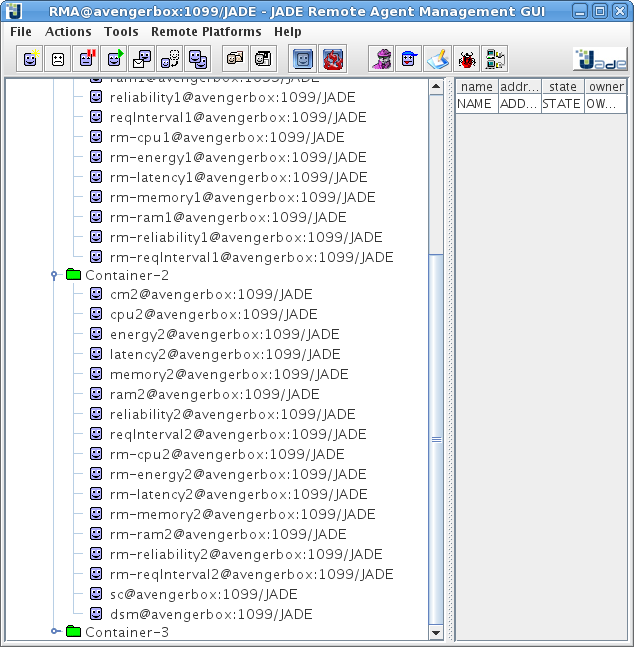
\includegraphics[scale=0.5]{etc/secondo.png}
\caption{Migrazione su secondo nodo}
\label{fig:secondo}
\end{center}
\end{figure}
Il nodo 3 è di tipo WIRELESS e quindi ha una energia limitata, il che implica un tempo di residenza per l'SC e il dsm molto più ridotto, in quanto l'indice raggiungerà rapidamente valori alti.
\begin{lstlisting}
Sono su Container-3
Context[cm1]--> cpu: 0.81155604, ram: 33.999382, memory: 51.11227, energy: 100.0, index: 19.762337
Context[cm2]--> cpu: 36.432972, ram: 58.424694, memory: 1.620206, energy: 84.948586, index: 26.705338
Context[cm3]--> cpu: 67.67117, ram: 95.22946, memory: 26.253895, energy: 49.21744, index: 58.74031
Associated with: cm3
Actual context--> cpu: 67.67117, ram: 95.22946, memory: 26.253895, energy: 49.21744, index: <58.74031>
Migration to cm1
Moving DSM to 1

Sono su Container-1
Context[cm1]--> cpu: 50.261562, ram: 62.669903, memory: 48.456142, energy: 100.0, index: 37.11915
Context[cm2]--> cpu: 1.1113803, ram: 6.8676476, memory: 18.00424, energy: 83.9486, index: 10.791573
Context[cm3]--> cpu: 83.216156, ram: 71.41142, memory: 32.01974, energy: 44.21744, index: 59.663654
Associated with: cm1
Actual context--> cpu: 50.261562, ram: 62.669903, memory: 48.456142, energy: 100.0, index: <37.11915>
\end{lstlisting}
L'energia del nodo 3 è scesa da 49 a 44 il che ha costretto la migrazione sul nodo meno carico, ovvero l'uno (WIRED). In seguito vi è stata anche una violazione del contratto ed è stata segnalata ad entrambi i nodi partecipanti al contratto, i quali dovranno adattarsi per evitare di ripetere la violazione.
\begin{lstlisting}
Violated with latency 23.106468 > 82.419365, reliability 41.978447 > 99.44324, reqInterval 79.21008 > 76.23332
\end{lstlisting}
Dal log si può notare che è stato il subscriber ad eccedere in rischieste, infatti il reqInterval è inteso come frequenza.
\section{Analisi dati}
In questa sezione verranno esposti e commentati i grafici relativi alla simulazione, in quanto molto più esplicativi dei log riportati sopra. Come passo fondamentale vengono ora riportati i grafici relativi agli indici.
\begin{figure}[H]
\begin{center}
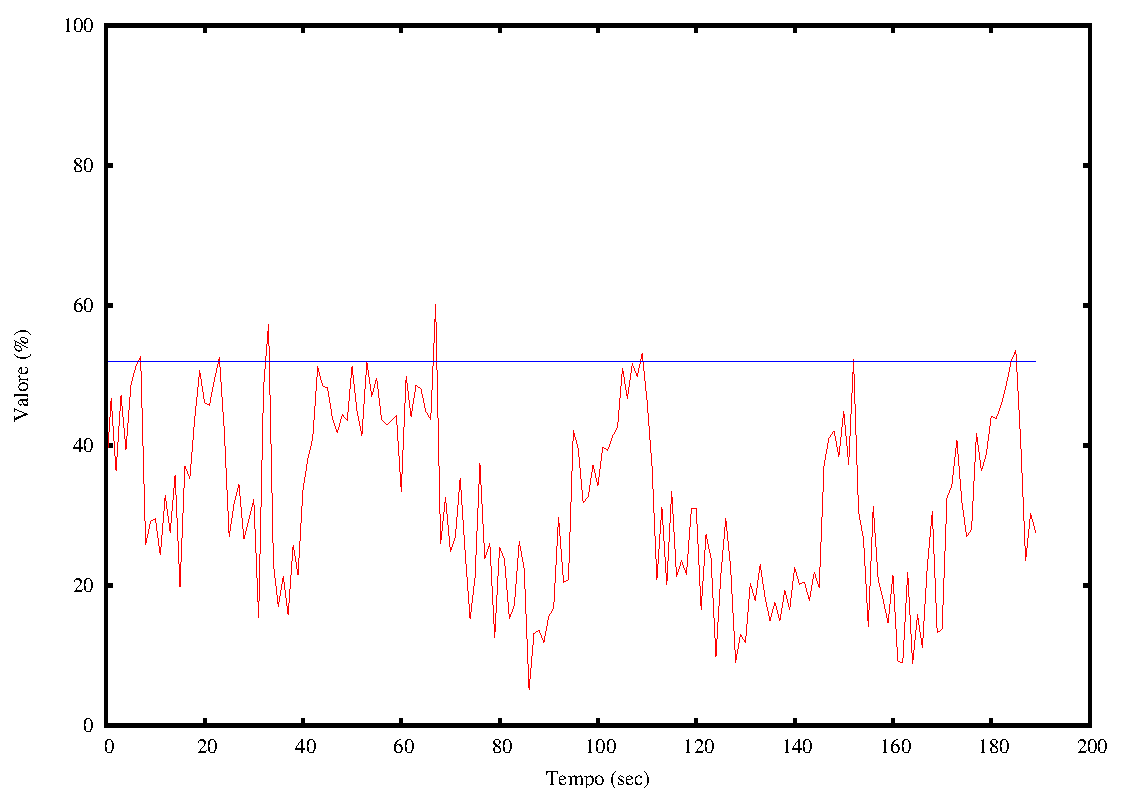
\includegraphics[scale=0.6]{etc/index1.pdf}
\caption{Indice primo nodo}
\label{fig:index1}
\end{center}
\end{figure}
\begin{figure}[H]
\begin{center}
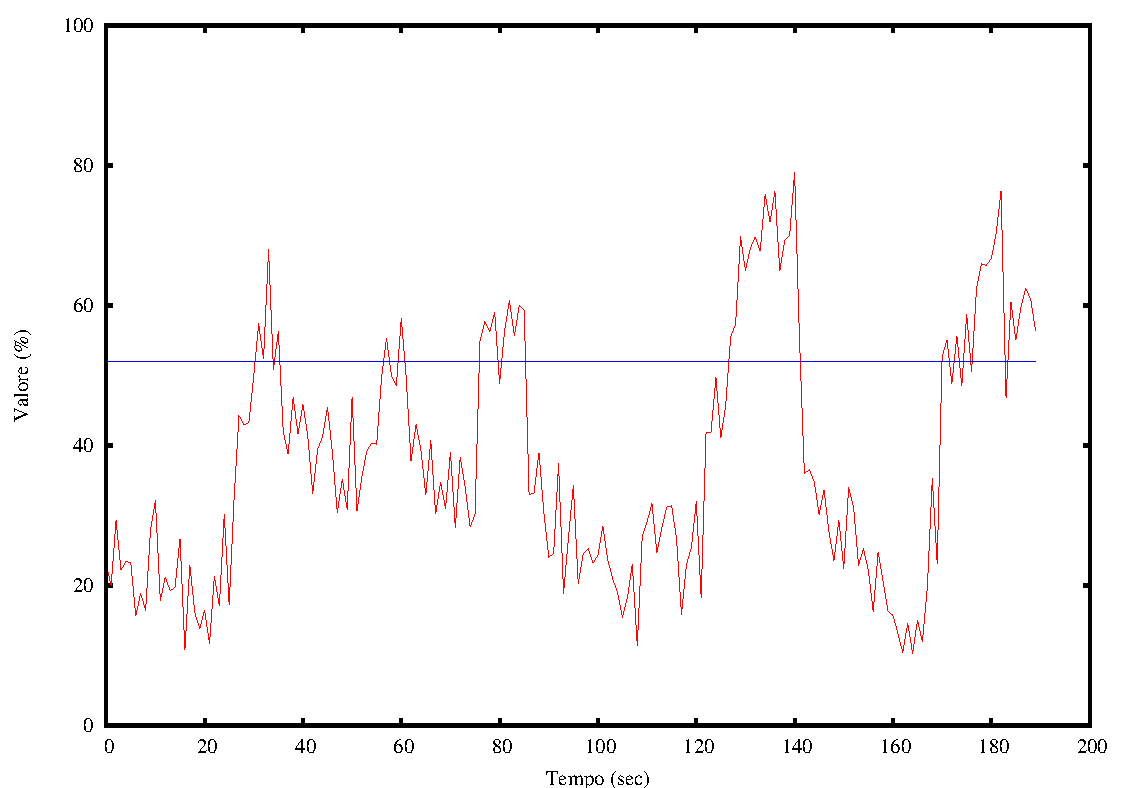
\includegraphics[scale=0.6]{etc/index2.pdf}
\caption{Indice secondo nodo}
\label{fig:index2}
\end{center}
\end{figure}
\begin{figure}[H]
\begin{center}
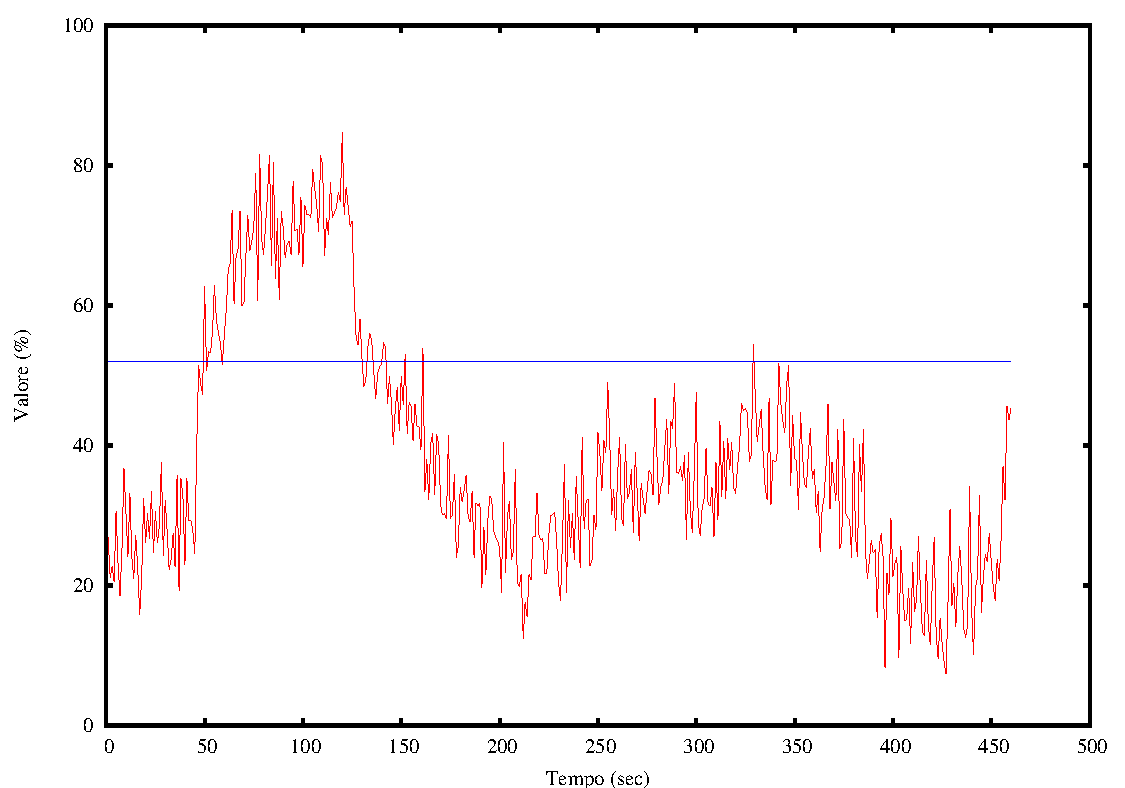
\includegraphics[scale=0.6]{etc/index3.pdf}
\caption{Indice terzo nodo}
\label{fig:index3}
\end{center}
\end{figure}
\begin{figure}[H]
\begin{center}
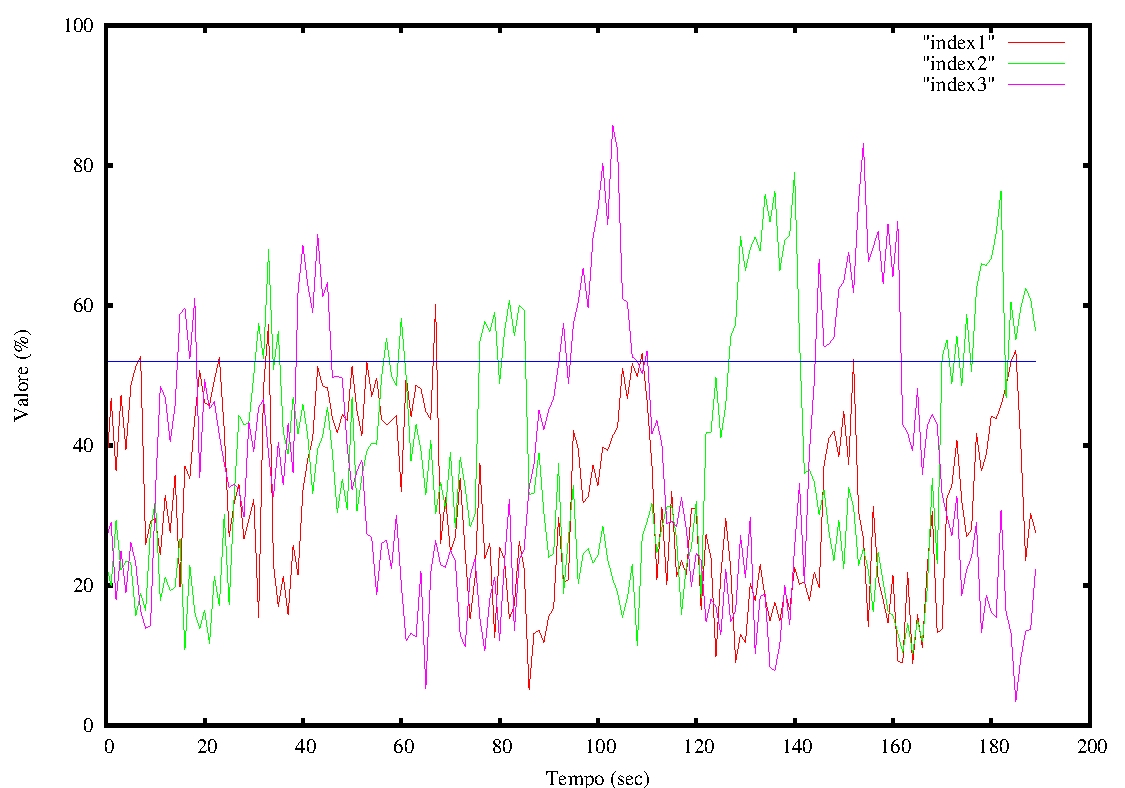
\includegraphics[scale=0.6]{etc/index.pdf}
\caption{Indice tutti i nodi}
\label{fig:index}
\end{center}
\end{figure}